\documentclass{article}
\usepackage{graphicx} % Required for inserting images

\usepackage[onehalfspacing]{setspace} % Increase line spacing
\usepackage[margin=2.5cm]{geometry} % Modify margins
% \usepackage{apacite} % APA citations
\usepackage{natbib}  % Better APA citation handling
\usepackage{subcaption}
\usepackage{booktabs}
\usepackage{amsmath}
\usepackage{amssymb}
\usepackage{enumitem}
\usepackage{multirow}
\usepackage{appendix}
\usepackage{float}

\title{Réseau de neurones DIY}
\author{Antoine Théologien - 21400184}
\newcommand{\program}{Master Informatique}
\newcommand{\parcours}{DAC}
\newcommand{\course}{Machine Learning}


\begin{document}

\begin{titlepage}
\makeatletter
\begin{center}
	\textsc{Sorbonne Université}
	\par \textsc{Sciences et ingénierie }
	\par \program

        \vfill
        \hrule height .08em \bigskip
	\par\huge\@title\bigskip
	\par\Large\@author\bigskip
	\hrule height .08em \normalsize

	\vfill
        \begin{figure}[H]
        \centering
        
\includegraphics[width=0.8\linewidth]{Logo_of_Sorbonne_University.svg.png}
        \label{fig:enter-label}
        \end{figure}
	\vfill

	\begin{tabular}{ll}
		\toprule
            Parcours : & \parcours\\
		Cours : & \course\\
		Date : & \@date\\
		\bottomrule
	\end{tabular}
	
	\vfill
\end{center}
\makeatother
\end{titlepage}

\section{Introduction}
Ce rapport est consacré au projet du cours Machine-Learning et consiste à réaliser une implémentation de réseau de neurones from scratch en Python, en essayant de reproduire au mieux le comportement de la très célèbre bibliothèque PyTorch. Dans celui-ci, les différents détails d'implémentation et les différentes expérimentations seront apportés. Le plan suivra celui de l'énoncé du projet, disponible dans l'archive. Le code source est également disponible dans cette dernière, ainsi que les notebooks contenant les différents tests réalisés.
\section{Prémisses}

Le projet se base ainsi sur une architecture modulaire, permettant d'assembler les différents éléments d'un réseau, facilitant la mise en place et le déploiement. On dispose ainsi de 2 classes principales qui serviront de classes mères pour la majorité des futures classes implémentées.
\subsection{Classe Module}
La première est la classe \textbf{Module}, qui, comme son nom l'indique, représente un module générique de notre réseau de neurones. Celle-ci contient toutes les méthodes permettant la bonne implémentation d'un réseau de neurones : forward, réinitialisation du gradient, backward, mise à jour des paramètres. Le diagramme de la classe est visible dans la figure \ref{fig:module}.

\begin{figure}[H]
    \centering
    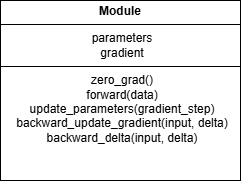
\includegraphics[width=0.4\linewidth]{module.png}
    \caption{Diagramme de la classe Module}
    \label{fig:module}
\end{figure}

La majorité des fonctions de cette classe ne sont pour l'instant pas implémentées, à l'exception des méthodes $zero\_grad$ et $update\_parameters$. Ainsi, dans la première, on commence par vérifier si la variable gradient n'est pas nulle, afin de s'assurer de pouvoir la manipuler. Si elle existe bien, on met à jour cette variable en mettant un zéro pour chaque paramètre contenu dans notre variable $parameters$. 
Dans $update_parameters$, on commence par vérifier cette fois-ci si les deux variables de notre classe sont bien définies, puis on met à jour la variable $parameters$ en soustrayant le vecteur de la variable $gradient$ à celui de nos paramètres, en veillant bien à multiplier celui-ci par le pas de gradient en paramètres.
Le reste des méthodes seront implémentées dans les classes filles qui héritent de cette classe abstraite.

\subsection{Classe Loss}
Cette seconde classe abstraite nous permet donc de disposer des méthodes pour implémenter les différentes fonction de perte que nous souhaiterions utiliser dans notre réseau de neurones. Elle ne dispose que de deux méthodes : $forward$, qui prend en paramètre deux entrées et calcule le coût, et la méthode $backward$, qui va nous permettre de calculer le coup du gradient par rapport à une entrée. Il n'y a donc pas besoin de les implémenter pour l'instant : il faudra le faire spécifiquement en fonction des fonctions de coûts que nous souhaitons mettre en place.

\section{Mon premier est ... linéaire !}
On commence donc par implémenter la perte MSE et un module linéaire, ce qui va nous permettre de réaliser tout d'abord des régressions linéaires.

\end{document}